
\chapter{Oscillazioni smorzate e forzate}


\section{Introduzione}

Oggetto di questa ricerca è lo studio delle oscillazioni smorzate e forzate di un pendolo. Studiando il variare delle oscillazioni al variare della frequenza operativa della forzante, si studierà il fenomeno della risonanza.

\subsection{Strumenti}
\begin{center}
\begin{tabular}{l|l}
Strumento & Precisione\\
\midrule
Calibro & $\pm 0.05$ mm\\ 
Sensore di rotazione & $\pm 0.00157$ rad\\ 
Alimentatore & $\pm 0.01$ V\\ 

\end{tabular}
\end{center}
L'attrezzatura utilizza è costituita da un disco metallico fissato ad una puleggia. La puleggia è messa in oscillazione da un filo alle cui estremità vi sono un oscillatore  elettromeccanico, che agisce come forzante, e un sistema di due molle. Al disco è possibile avvicinare e allontanare un magnete, che ha la funzione di smorzare il moto.

\section{Oscillazioni libere}

Si pone in oscillazione il disco, con il magnete  posizionato lontano e l'oscillatore elettromeccanico spento. Un sensore di posizione misura lo spostamento angolare; il sensore è collegato ad un computer, ed il programma DataStudio traccia in tempo reale il grafico dello spostamento angolare in funzione del tempo. Si interpolano dunque i dati con una funzione sinusoidale per determinare il periodo, e si ricava: $$T=1.47\pm0.02\ s$$ L'errore riportato è quello che il programma stesso attribuisce alla rilevazione, ed è determinato dalla precisione degli strumenti di rilevamento e dall'interpolazione dei dati.\\
Dal periodo possiamo ricavare il valore della pulsazione $\omega$, dalla relazione:
\begin{equation}\label{omepe}
\omega=\frac{2\pi}{T}
\end{equation}
e si ottiene:
$$\omega=4.272\ rad/s$$
con un errore dato dalla propagazione di quello su T:
$$\sigma_{\omega}=2\pi\left(|\frac{-1}{T^2}|\right)\sigma_T=0.06\ m/s$$
\section{Oscillazioni smorzate}

Si avvicina il magnete al disco metallico. Il moto oscillatorio risulterà così smorzato per effetto delle correnti di Focault.
I dati raccolti dal sensore sono stati interpolati con la funzione
\begin{equation}\label{eq:theta}
\theta (t) = A_0 e^{- \gamma t} \sin(wt+\phi)+\theta_0
\end{equation}
al fine di determinare i parametri liberi; i valori ottenuti sono riportati di seguito in tabella.\\

$$T=1.45\ s$$

\begin{center}
\begin{tabular}{l|l|l}
Parametri & Valore ricavato & $ \pm \sigma$ \\
\midrule
$A_0$ & 3.08 rad & 0.020\\
$\gamma$ & 0.197 $m^4/kg$& 0.0019\\
$\omega$ & -4.27 rad/s& 0.0019\\
$\phi$ & 1.93 rad & 0.0069 \\
$\theta_0$ & -1.53 rad& 0.0019 \\
\end{tabular}
\end{center}

A questo punto, noti $\omega$ e $\gamma$, è possibile calcolare $ \omega_0 $, cioè la pulsazione per le oscillazioni libere, tramite l'equazione:
\begin{equation}\label{eq:omega}
\omega = \sqrt{\omega_0^2 - \gamma^2}
\end{equation} da cui:
$$\omega_0 = 4.275\ rad/s$$

Confrontandolo con il valore che avevamo ricavato interpolando direttamente il grafico delle oscillazioni libere si nota che i due non coincidono, ma che quello misurato dal periodo delle oscillazioni libere è minore di quello ricavato dalla formula: infatti, essendo un sistema reale, tra le sue parti sono presenti degli attriti che smorzano le oscillazioni.

\section{Oscillazioni smorzate-forzate}

Mantenendo il magnete vicino al disco, abbiamo messo in azione l'oscillatore elettromeccanico, che fornisce la componente forzante. Variando il voltaggio dell'alimentatore,  la frequenza di rotazione dell'oscillatore cambia: abbiamo così cercato la frequenza di risonanza del sistema.
Poiché il periodo dell'oscillatore armonico coincide con quello della forzante, abbiamo potuto leggere direttamente il periodo dal valore restituito dalla fotocellula. Dopo aver atteso che il sistema si fosse stabilizzato, abbiamo interpolato i dati con il programma DataStudio, secondo la funzione
\begin{equation} \label{A}
A(\omega) = \frac{M_0}{\sqrt{ ({\omega_0}^2-\omega^2)^2 + 4\gamma^2\omega^2}}
\end{equation}

ed abbiamo ricavato così i valori corrispondenti ai parametri liberi $M_0$, $\gamma$ e $\omega_0$. 

Tale procedura è stata ripetuta spostando il magnete a distanze differenti dal disco.
\\
Di seguito sono riportati i dati raccolti e i rispettivi grafici. I primi dati si riferiscono alle condizioni del sistema smorzato (prima dell'accenzione dell'oscillatore elettromeccanico), e riportano il periodo corrispondente e i parmaetri liberi ricavati dall'interpolazione con la \ref{eq:theta}. Subito sotto il periodo si trova invece il valore di $\omega_0$ ottenuto dalla \ref{eq:omega}. \\In tabella sono trascritti i valori dei periodi letti dalla fotocellula al variare della forzante, il corrispondente $\omega$ (dato dall'equazione \ref{omepe}), e il valore dell'ampiezza ottenuto dall'interpolazione con una funzione sinusoidale. Di fianco alle tabelle si trovano i valori ottenuti dall'interpolazione con la funzione \ref{A}. Il grafico illustra l'andamento dell'ampiezza al variare della pulsazione: i picchi corrispondono alla condizione di risonanza.\footnote{Quando dalle interpolazioni emergevano errori di un ordine di grandezza molto piccolo, abbiamo evitato di trascriverli, ritenendoli trascurabili.}

\subsubsection{4.80mm}

\textit{Oscillazioni smorzate}
I dati relativi alle oscillazioni smorzate con il magnete a 4.80 mm si trovano riportati nella sezione "Oscillazioni smorzate".
\textit{Oscillazioni forzate}
\begin{center}

\begin{tabular}{c c}

\begin{tabular}{c | c | c}
\textbf{Ampiezza ($rad$)} & \textbf{Periodo ($s$)} & \textbf{Pulsazione ($rad/s$)}\\
\midrule
0.89 & 5.45 & 1.15\\
0.94 & 4.78 & 1.31\\
1.05 & 3.57 & 1.75\\
1.09 & 3.19 & 1.97\\
1.30 & 2.46 & 2.55\\
1.30 & 2.59 & 2.42\\
1.84 & 2.06 & 3.05\\
1.91 & 1.90 & 3.31\\
3.42 & 1.70 & 3.69\\
6.35 & 1.59 & 3.95\\
1.19 & 1.14 & 5.51\\
\end{tabular}

& \hspace{1cm} 

\begin{tabular}{c}
$ \omega_0 = 4.25\ rad/s $\\
\\
$ \gamma = 0.193\ s^{-1}$\\
\\
$ M_0 = 15.3\ s$\\
\end{tabular} 

\end{tabular}

\end{center}
 
\begin{center}

\includegraphics[scale=0.75]{"../grafici/Magnetea48mm"}


\end{center}
 
 
\subsubsection{2.80mm}

\textit{Oscillazioni smorzate}

\begin{center}

\begin{tabular}{c c}

\begin{tabular}{c}
$T_{smorzate}=0.877\ s$\\
\\
$\omega_{0} = 4.297\ rad/s$\\
\end{tabular}

& \hspace{2cm}

\begin{tabular}{c}
$A_0 = 3.4 \pm 0.020\ rad$\\
\\
$\gamma =  0.636 \pm 0.0057\ m^4/kg $\\
\\
$\omega = -4.25  \pm 0.0064\ rad/s $\\
\\
$\phi =  2.38 \pm 0.0076\ rad $ \\
\\
$\theta_0 = -0.57 \pm 0.0038\ rad $\\
\end{tabular}

\end{tabular}

\end{center}

\textit{Oscillazioni forzate}

\begin{center}

\begin{tabular}{c c}

\begin{tabular}{c | c | c}
\textbf{Ampiezza} ($rad$) & \textbf{Periodo} ($s$) & \textbf{Pulsazione} ($rad/s$)\\
\midrule
1.68 & 2.00 & 3.14\\
2.95 & 1.63 & 3.85\\
3.22 & 1.44 & 4.36\\
2.17 & 1.30 & 4.83\\
1.20 & 1.15 & 5.46\\
1.67 & 1.24 & 5.06\\
0.99 & 1.10 & 5.71\\
0.68 & 0.98 & 6.40\\
0.51 & 0.89 & 7.06\\
0.26 & 0.74 & 8.49\\
\end{tabular}

& \hspace{1cm}

\begin{tabular}{c}
$ \omega_0 = 4.26\ rad/s $\\
\\
$ \gamma = 0.543\ s^{-1} $\\
\\
$ M_0 = 15.6\ s$\\
\end{tabular}

\end{tabular}

\end{center}

\begin{center}
\includegraphics[scale=0.75]{"../grafici/Magnetea28mm"}

\end{center}


\subsubsection{1.00mm}

\textit{Oscillazioni smorzate}

\begin{center}

\begin{tabular}{c c}

\begin{tabular}{c}
$T_{smorzato}=2.15\ s$\\
\\
$\omega_{0} = 4.291\ rad/s $\\
\end{tabular}

& \hspace{2cm}

\begin{tabular}{l}

$A_0 = 18600 \pm 1300\ rad$ \\
\\
$\gamma= 1.50 \pm 0.0011\ m^4/kg$\\
\\
$\omega = 4.02 \pm 0.0077\ rad/s$\\
\\
$\phi =  26.3 \pm 0.0046 \ rad/s$ \\
\\
$\theta_0 = 0.055 \pm 0.0016\ rad$ \\
\end{tabular}

\end{tabular}

\end{center}

\textit{Oscillazioni forzate}

\begin{center}

\begin{tabular}{c c}

\begin{tabular}{c | c | c}

\textbf{Ampiezza} ($rad$) & \textbf{Periodo} ($s$) & \textbf{Pulsazione} ($rad/s$)\\
\midrule
1.33 & 2.01 & 3.12\\
1.42 & 1.85 & 3.39\\
1.45 & 1.67 & 3.76\\
1.18 & 1.31 & 4.79\\
1.31 & 1.39 & 4.52\\
1.47 & 1.54 & 4.07\\
0.76 & 1.09 & 5.76\\
0.88 & 1.19 & 5.28\\
1.01 & 1.22 & 5.15\\
0.49 & 0.93 & 6.75\\
0.65 & 1.03 & 6.10\\
0.39 & 0.85 & 7.39\\

\end{tabular}

& \hspace{1cm}

\begin{tabular}{c}
$\omega_0 = 4.37\ rad/s $\\
\\
$\gamma = 1.40 \pm 0.14\ s^{-1}$\\
\\
$M_0 = 17.1 \pm 1.4\ s$\\
\end{tabular}

\end{tabular}

\end{center}

\begin{center}
\includegraphics[scale=0.75]{"../grafici/Magnetea10mm"}
\end{center}

\section{Conclusioni}

\begin{center}
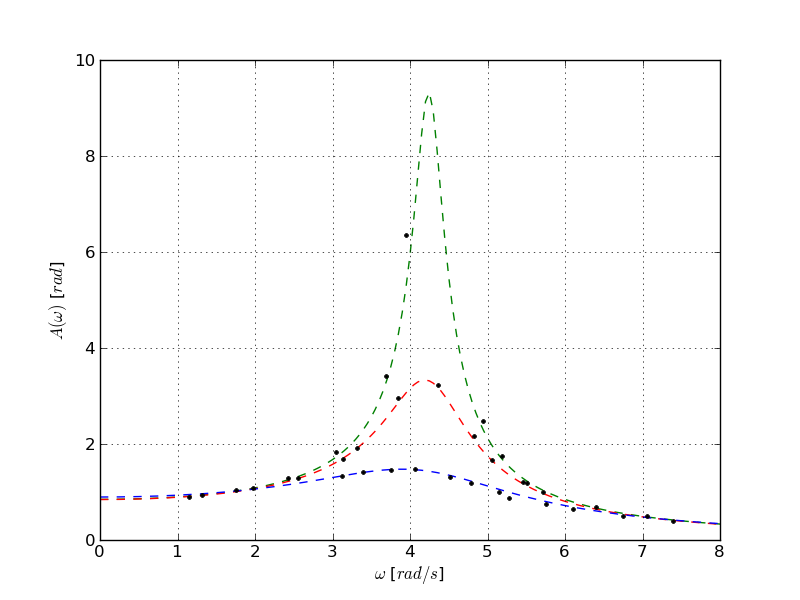
\includegraphics[scale=0.85]{../grafici/risonanza}
\end{center}

Sovvrapponiamo le curve trovate in precedenza, e vediamo verificarsi la condizione di risonanza.
Con l'approssimarsi di $\gamma $ a zero, la curva blu ha infatti $\gamma=1.40\ s^{-1}$, la rossa $\gamma=0.543\ s^{-1}$, la verde $\gamma=0.193\ s^{-1}$,  il valore dell'ampiezza tende a $+\infty$.

\begin{center}
\begin{tabular}{c c}

\begin{tabular}{c|c|c|c}
&$\omega_0\ Libere\ (rad/s) $ & $\omega_0\ Smorzate\ (rad/s) $ & $\omega_0\ Smor. Forzate \ (rad/s) $\\
\midrule
4.80mm&4.27 &4.25 & 4.25 \\
2.80mm&4.27 & 4.30 & 4.26 \\
1.00mm&4.27 &4.29& 4.37 \\
\end{tabular}
&
\begin{tabular}{c|c}
$\gamma_0\ Forzate $ & $\gamma_0\ Smorzate $\\
\midrule
1.40 &1.50\\
0.543 &0.636\\
$\sim 0$ &0.193\\
\end{tabular}
\end{tabular}
\end{center}

Pur trattandosi dello stesso parametro, ricavandolo attraverso interpolazioni e condizioni fisiche diverse, si ottengono valori leggermente differenti. All'aumentare dello smorzamento i valori si discostano maggiormente fra di loro. 


